% Slide 18: Risk & Mitigation
\begin{frame}{Risk \& Mitigation}
    \framesubtitle{Proactive Risk Management}

    \begin{center}
        \begin{tabular}{p{4cm}p{6cm}}
            \toprule
            \textbf{Risk} & \textbf{Mitigation Strategy} \\
            \midrule
            \textcolor{red}{Market Competition} & Strong IP portfolio, continuous innovation, and focus on customer success \\
            \midrule
            \textcolor{red}{Technology Changes} & Modular architecture, active R\&D, and partnerships with leading tech providers \\
            \midrule
            \textcolor{red}{Scaling Challenges} & Experienced team, proven processes, and strong operational infrastructure \\
            \midrule
            \textcolor{red}{Customer Concentration} & Diversified customer base across industries and geographies \\
            \midrule
            \textcolor{red}{Regulatory Changes} & Compliance-first approach, legal expertise, and industry monitoring \\
            \bottomrule
        \end{tabular}
    \end{center}

    \vspace{0.5cm}

    \centering
    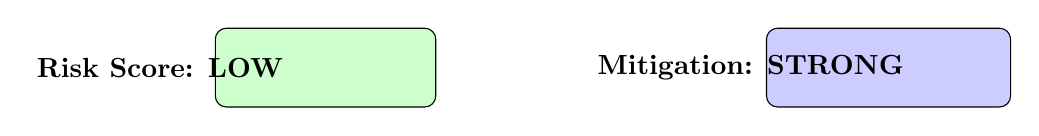
\begin{tikzpicture}
        \draw[fill=green!20,rounded corners] (-1.8,0) rectangle (1,1);
        \node at (-2.5,0.5) {\textbf{Risk Score: LOW}};

        \draw[fill=blue!20,rounded corners] (5.2,0) rectangle (8.3,1);
        \node at (5,0.5) {\textbf{Mitigation: STRONG}};
    \end{tikzpicture}
\end{frame}